\documentclass[a4paper,12pt]{scrartcl}
\usepackage[utf8]{inputenc}
\usepackage{makeidx}
\usepackage{amsmath,amsfonts,amsthm}
\usepackage[english]{babel}
\usepackage[square,numbers]{natbib}
\usepackage{hyperref}
\bibliographystyle{alphadin}
\usepackage{graphicx}



\begin{document}

\begin{titlepage}
\begin{center}


\vspace*{1cm}

\bigskip
\bigskip
\large


\bigskip
\bigskip
\bigskip
\bigskip
\bigskip
\bigskip
\bigskip
\bigskip
\bigskip
{\LARGE \bfseries The Toyota Management System   }\\
{\bfseries -- Guiding principles and main tools --}

% Author -----------------------------------------------------------------------

\bigskip
\bigskip
\bigskip
\bigskip

Toni Pfeiffer \\

\bigskip
\bigskip
\bigskip
\bigskip
\bigskip
\bigskip
\bigskip
\bigskip
\bigskip
\bigskip
\bigskip
\bigskip
\bigskip
\bigskip
\bigskip
University of Leipzig \\
\bigskip
\bigskip
Faculty of Mathematics an Computer Science \\
\bigskip
Seminar Complex Systems and Co-Operative Actions \\
\bigskip
\bigskip
\bigskip
\bigskip
\bigskip
\bigskip
\bigskip
\bigskip
\bigskip
\bigskip
\bigskip
\bigskip
\bigskip
\bigskip
\bigskip
\bigskip
Leipzig, \today

\end{center}

\bigskip
\bigskip
\bigskip
\bigskip
\bigskip

\end{titlepage}

\clearpage
\tableofcontents
\clearpage
\clearpage
\addcontentsline{toc}{section}{List of Figures}
\listoffigures
\clearpage

\section{Introduction}

This seminar paper refers to the book "The Toyota Way - 14 Management Principles of the World's Most Successful Automotive Company" by Jeffrey K. Liker. Jeffrey Liker observed the company for 20 years and summarized his knowledge about it in the book. He analyzed Toyota's success and discovered 14 methods that enabled Toyota to become the most successful automotive company in the world. To understand Toyota's success, it is necessary to look at the history of the company. This will be done in the next chapter. The Toyota Production System, another component of success, will be described in Section 2.1. Here we will focus on the management methods that describe the holistic approach. The individual principles were divided by Liker into 4 categories, also called the 4 P's. These categories can be thought of as a pyramid, shown in Fig. \ref{4P}. Problem solving is the top of the pyramid. The most important is the foundation, the philosophy of the company. This philosophy runs through all management levels and eras. Starting with the founding Toyoda family, which is described in more detail below.

\clearpage
\section{History}

    To understand Toyota's success, you have to look at the company's history. It all began with Sakichi Toyoda. He was a Japanese carpenter, just like his father. He was considered a tinkerer and inventor from a young age. He began by making mechanical looms. Being tireless in perfecting things, he built an automatic loom. To do this, he and his son bought an old steam engine and combined it with the looms. Together they were successful and now wanted to enter the emerging automotive industry. However, they still needed some start-up capital, which the son, Kichiro Toyoda, obtained in Great Britain. He sold their patent for the automated loom there. With a starting capital of now 100,000 pounds, the two set to work to produce their first car. In 1937, the father decided to stay with his looms and the son, Kichiro, founded Toyota. 
    
    Toyota, of course, benefited from the general industrial boom, as did many other companies, including Siemens and General Motors. During this period, the professions of managers and engineers developed. The vision of many American companies at that time was to create an organization that ran like a machine. Toyota took a different approach, that of a living organization. What this means will be examined in more detail below. A big difference to the American car manufacturers is also that they aim at quantity. Toyota tries to ensure high quality even far away from the assembly line work and was thus one step ahead of the competitors from America.
    
    Fortunately, Toyota came out of World War II relatively unscathed. What caused more trouble for the company was the continuing inflation. Kichiro's goal was to lay off as few workers as possible. He succeeded for a while, as he and his managers waived their salaries. But at some point, he was forced to lay off employees. Of course, this led to resentment among the workforce and he himself felt it was a great personal defeat. As a result, he left Toyota and put his cousin Eiyi Toyoda in charge of the company. He was very impressed by the US productivity in the Ford and General Motors car plants. After several visits, he returned from the U.S. and gave his plant manager, Ono Taiichi, the task of making Toyota's plants even more productive than those of the Americans.
    
    
    
    
\subsection{Toyota Production System}
    
    The plant manager, Ono Taiichi, now achieved the feat and developed the Toyota Production System. Jeffrey K. Liker describes the system in his book as a house as shown in Fig. \ref{TPS}. It is important to note that the house only holds together if all its components hold together. Thus, the Toyota Production System is an interplay of many principles and instruments. The foundation is laid by the Toyota philosophy, visual management, standardized processes and balanced production methods. The individual principles will be described in more detail in the course of this seminar paper. The supporting pillars are the just-in-time process and the Jidoka process. The just-in-time process is concerned with the punctual delivery of add-on parts and the safeguarding of supply chains. The aim is to avoid storage costs for these parts. The basic prerequisite for this is a continuous flow, a so-called pull system and the possibility of a quick exchange of the production line. However, only individual parts of the production line are exchanged so that a different end product is obtained. A decisive role in the just-in-time process is played by the supplier. That's why people and the team are at the center of the company. The other supporting pillar is the Jidoka principle. Here Toyota is concerned with ensuring immediate quality and not having to make many improvements. They accomplish this by applying the Andon Principle. This means that when a defect occurs, the entire process should be stopped to look for the defect first, no matter how small it is. Another important point is the elimination of non-value elements. This involves avoiding the 3 M's, muda, mura and muri. 
    
    When all these points work together, the best quality can be achieved at the lowest cost, the fastest time, the highest safety and the best work ethic. Ono Taiichi has basically developed this system for the field of production. But it has become part of Toyota's DNA so that it can be applied in all other areas as well.


\begin{figure}[h] 
  \centering
     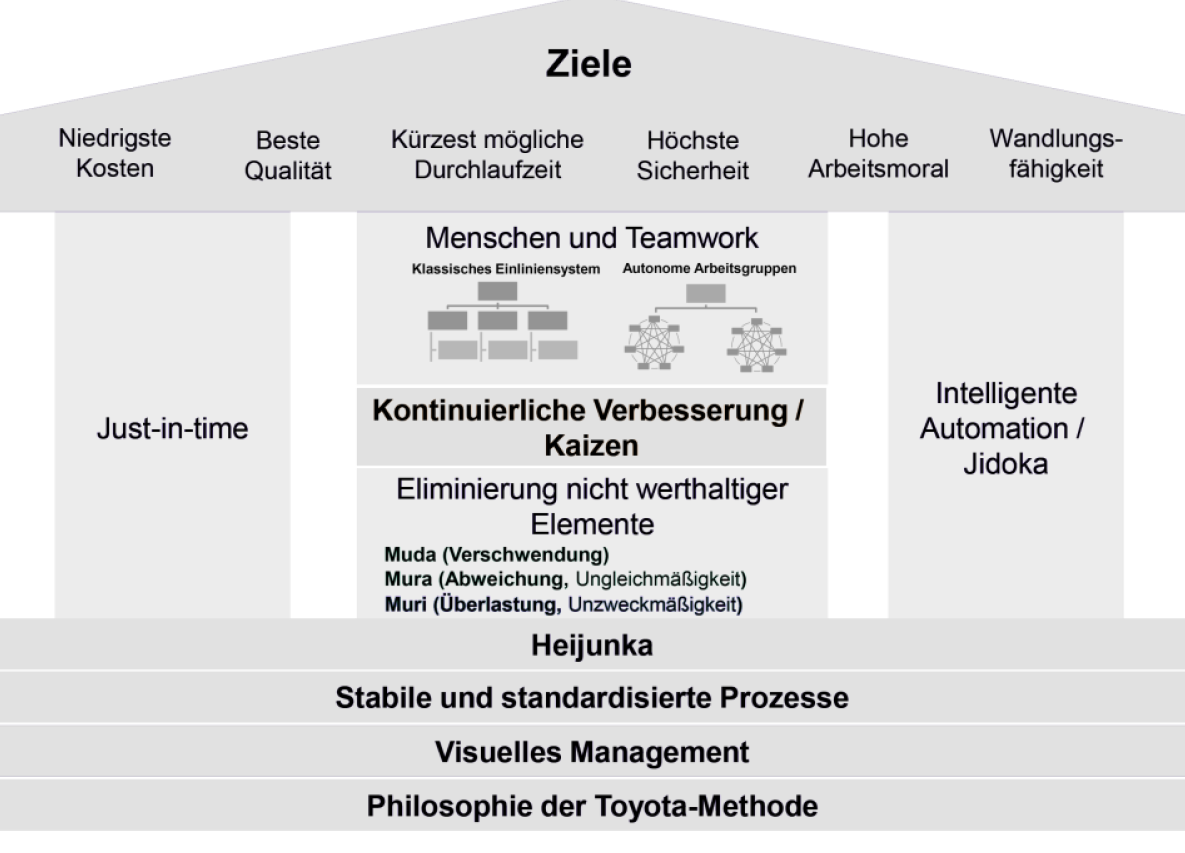
\includegraphics[width=0.7\textwidth]{TPS.png}
  \caption{Toyota Production System}
  \label{TPS}
\end{figure}

\clearpage

\section{Principles}

Liker now found that these principles are applied throughout the company and thus formulated the Toyota Way. This is made up of the 14 principles he describes in his book. He divides them into 4 categories. These 4 categories can also be described as the 4 P's. Together they form a pyramid as shown in Fig. \ref{4P}. At the top is problem solving. Here, kaizen and genchi genbutsu are applied. These are Japanese terms used at Toyota to describe the principles. The second P stands for people and partners. Here, Liker has found that Toyota hires only certain executives and chooses its suppliers wisely. The third P is process. This is where most of the principles are found. The fourth P is the most important principle. All decisions are based on philosophy. Toyota is primarily concerned with long-term thinking. What the philosophy and the other principles aim at in more detail is explained in the following chapters.

\begin{figure}[h] 
  \centering
     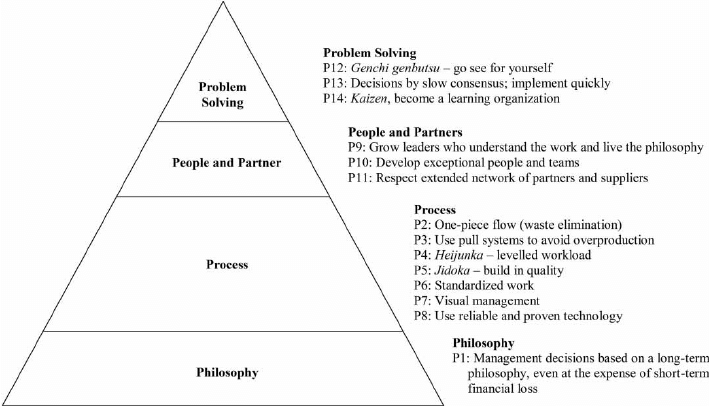
\includegraphics[width=0.9\textwidth]{4P.png}
  \caption{4P model of the Toyota Way}
  \label{4P}
\end{figure}

\subsection{Philosophy}



\subsubsection{1. Principle: Long-term thinking}

Toyota's guiding principle in philosophy is "Make a long-term philosophy the basis of your management decisions, even if it comes at the expense of short-term profit goals." A good example of this is the story of the Toyota plant in Long Beach California. In the 1960s, the U.S. imposed import duties of 30\% on trucks. Since Toyota wanted to continue exporting trucks to the US a solution had to be found. Other companies found a way and sent the truck without the bed and the bed separately to the USA. Since these counted as components, no duties had to be paid on them. Toyota used the same trick, but manufactured its truck beds directly on site. This is namely one of the philosophy principles, strengthen the local economy of a region. This plant now ran very well for several decades. Shortly before its 30th anniversary, Toyota wanted to close it down and outsource to Mexico, where wages were cheaper. Thus Toyota would have expected a short-term profit, which however would have been taken at the expense of the long-term goals. The plans were scrapped and the company is now very proud of the plant, which now produces fuel cells for trucks.
Liker describes in his book that Toyota's philosophy is aimed at 3 main points. One is value generation for the customer, society and the economy. He also finds 7 points that summarize the philosophy well:


\begin{itemize}
    \item We honor the language and spirit of each country's legislation and pay attention to open and fair corporate activities in order to be a good citizen of the world community.
    \item We respect the customs and traditions of each country and contribute to the economic and social development through corporate activities in our respective local communities.
    \item We are committed to environmentally sound and safe products and to improving the quality of life, at each site and in all our activities.
    \item We invent and develop advanced technologies and provide outstanding products and services that meet the needs of our customers worldwide.
    \item We foster a corporate culture that enhances the creativity of each individual and the value of teamwork, while building mutual trust and respect between the workforce and management.
    \item We pursue growth in harmony with the global community through innovative management.
    \item We collaborate with business partners in research and development to create stable, long-term growth and mutual benefit, while keeping ourselves open to new partnerships.
\end{itemize}


\clearpage

\subsection{Process}

The second P that Liker describes in his book is process. Here the elimination of waste, also called muda, is in the foreground. Instruments that can build on this are for example the pull system or the possibility to use only reliable technologies. This category is divided into 7 principles which will be looked at in more detail below. 

\subsubsection{2. Principle: One-Piece Flow}

The main focus of the One-Piece-Flow is the elimination of waste. It is important to find out what are value-adding activities and what are not. It can happen that a process consists of 90\% waiting and 10\% value adding activities. If you can eliminate this 90\%, it is possible to reduce a process that took days to a few hours. According to Liker, these wastes can be the following:

\begin{itemize}
    \item overproduction
    \item waiting times
    \item unnecessary transports
    \item too many or wrong process steps
    \item excess stock
    \item unnecessary movements
    \ errors
    \item unused creativity potential of employees
\end{itemize}

If you are now able to eliminate these, as Toyota manages to do time and again, you can reap the following benefits:

\begin{itemize}
    \item Quality improvement\\
    It is much easier to achieve high quality in a one-piece flow. Each assembler or machine operator acts as an inspector and works to solve problems that arise at his or her workstation, rather than passing them on to the next stage of processing. If defects are overlooked at a workstation, however, it doesn't take long for them to be discovered so the problem can be diagnosed and corrected as quickly as possible.
    \item Real flexibility\\
    When machines are used for a specific vehicle line, they can no longer be flexibly used for other purposes. But if the lead times to manufacture a product are very short, this is precisely what would create greater flexibility in responding to customer needs. Instead of realigning a system and waiting weeks for the product to finally be ready, new orders can be fulfilled in a matter of hours with short lead times. Retooling to a different product mix to accommodate a change in customer demand can be done almost immediately.
    \item Productivity increase\\
    The reason productivity seems to be higher when your operation is divided into departments has to do with the fact that each department is measured by the utilization of its machines and employees. But in fact, with the batch-and-queue method, it's very difficult to determine how many employees are really needed to produce a given number of units because productivity is not measured by the value-added work. Who knows how much productivity is lost by "stretching" employees to produce surplus goods that then have to be stacked in warehouses? How much time is lost by having to track defective parts and components and rework finished products? In a one-piece flow cell, there is little non-value added activity such as moving materials from one workstation to the next. It becomes immediately apparent who is overloaded and who is underutilized. It is easy to calculate the proportion of value-added work and then calculate how many employees are needed to achieve a given production rate. In every single case in which the Toyota Supplier Support Center converted suppliers' mass production to TPS, an increase in labor productivity of at least 100 percent was achieved.
    \item Reduction in required plant floor space\\
    Setting up machines by department creates large unused open spaces between each machine. The biggest waste of space, however, comes from intermediate storage with stacks of parts and components. In a cell, all process steps are arranged close together, and there is hardly any intermediate storage. By making better use of plant space, the otherwise unavoidable increase in capacity can be avoided.
    \item Increase in safety\\
    Smaller quantities of parts meant eliminating the need for large forklifts, which often lead to accidents. It also meant lifting and transporting smaller containers of material. So accidents related to lifting heavy weights would also no longer occur. Safety increased with a focus on process flow - even without a specific focus on safety.
    \item Increase in work morale\\
    In a one-piece flow, employees do more value-added work and see the results of their work immediately. This provides a sense of accomplishment, creating job satisfaction.
    \item Reduces the cost of inventory\\
    In this way, they free up dead capital for other investments. It also eliminates the cost of inventory. Inventory obsolescence also decreases.
\end{itemize}

\clearpage

\subsubsection{3. Principle: Pull-System}

The next principle Liker puts in the process category is the use of the pull system. The difference between pull and push is the direction of the supply chains.In the push method, the supplier manufactures parts and sends them to Toyota after production. They cannot process the quantity of parts directly and store them temporarily. It is obvious that this leads to problems, especially in warehousing. Toyota therefore uses the pull system. Whereby they determine when a part is to be delivered. Thus the supplier starts to produce the part as soon as the order from Toyota is received. This approach avoids backlogs and requires a decentralized control system. A steady flow of material is also important. Therefore, Toyota never orders more than it needs and can thus implement its just-in-time approach. 

\subsubsection{4. Principle: Heijunka}

The 4th principle is called Heijunka. Here Toyota is concerned with the balance of the workflow. Liker describes this with the 3 M's, muda, mura and muri. Muda has already been described. Muri means overload of man and machine. Mura means imbalance. These 3 must not gain the upper hand so that the system can remain balanced. An important point is not to process the orders after they have been received. Toyota looks at the orders over a period of time and then adjusts the manufacturing sequence based on that. The main focus is to keep the load on man and machine as low as possible. An important point here is flexibility. Especially that of the machines. For example, Toyota has succeeded in shortening the changeover times of production lines to such an extent that a line can be switched from the manufacture of one product to another while the line is still in operation. This can be thought of as a pit stop in Formula 1. Thus, the "build to order" becomes a "change to order".

\subsubsection{5. Principle: Jidoka}

The 5th principle is called Jidoka and describes Toyota's culture of delivering quality first time and not having to make constant improvements. The entire process is usually interrupted when an error occurs in order to ensure the quality at the first go and not to be dependent on unnecessary rework. Liker crystallizes 4 steps in this process:

\begin{itemize}
    \item Make your own picture
    \item Perform a detailed analysis
    \item Use the andon principle 
    \item Ask 5 times why
\end{itemize}

The andon principle is a way to indicate the errors in the production. Like an alarm light in a production line, which shows you where the problem is.

\subsubsection{6. Principle: Standardized work}

The 6th principle is the standardization of the work steps. The goal of all production steps is, of course, to improve production. This can only be achieved if the processes have a standard way that the employees carry out. This is the same as in golf. If you can't even hit the ball by default, you can't improve your golf swing. 
Toyota's path to standardization is as follows. They try to involve every employee in determining such work standards. For this purpose, so-called pilot teams are formed, whose task is to set new standards. Such a pilot team consists of employees from all shifts and departments. Every 3-4 years the occupation of such a team changes. This way everyone is able to set the standards and there are no complaints when new standards are introduced, because each department has a say. Thus, Toyota's way is precise enough to set such standards, but also leaves enough room for the employees to be creative.

\subsubsection{7. Principle: Visual Management}

Visual management describes the 7th principle of the Toyota Way. This is divided into the 5 S's:

\begin{enumerate}
    \item Seiri: Sort\\
    Sort all things and keep only what you really need and dispose of everything else.
    \item Seiton: orderliness \\
    A place for everything and everything in its place.
    \item Seiso: Cleanliness\\
    When cleaning, an inspection usually takes place at the same time, alerting you to irregularities and impending defects that can lead to quality degradation or machine breakdowns.
    \item Seiketsu: Standardize/Create Rules \\
    Develop systems and procedures to monitor compliance with the first three S's.
    \item Shitsuke: Self-discipline \\
    Maintaining a stable workflow is a continuous improvement process. Discipline, of course, is the hardest process as everyone knows themselves
\end{enumerate}

\subsubsection{8. Principle: Use only reliable technology}

The last principle of the Processes category is the guiding principle that Toyota only uses technologies that are reliable. The fact is that Toyota puts a lot of thought into a new technology, such as new software, before it is introduced. Liker described the process as follows. When a new technology is launched, Toyota starts with a comprehensive analysis. They form a pilot area in the department where the new technology could be introduced. In this pilot area, however, they do not test the technology, but first apply all other instruments and tools for productivity improvement that Toyota has at its disposal up to that point. If the methods do not lead to improvements, the introduction of the technology can be considered in more detail. However, it must be consistent with the preceding principles. This technology should put people above machines, preserve the consensus principle, avoid waste, be flexible, visual and intuitive. This decision involves everyone in the process. The decision maker is then the engineer on site who will oversee the new technology. 

\subsection{People}

The 3rd category Liker describes in his book he calls people and partners. Toyota is primarily concerned with team and network building as well as with the managers. How Toyota selects these and what distinguishes them is described below. 

\subsubsection{9. Principle: Leaders}

The most important thing for the managers is that they have internalized the company philosophy and that they exemplify and convey this to others. Toyota makes sure that they are trained internally instead of recruiting a new employee. An important part of the Toyota management is the chief engineer. This person is the interface between the department and the production line. As a critical interface between innovation, management level and customer satisfaction, they have the backing of top management. The chief engineer has the ear of top management, which is committed to providing him or her with all the resources necessary for success. 
In observing many managers, Liker has found that almost all have this in common:

\begin{itemize}
    \item Focus on the long-term goal
    \item No deviation from the core of Toyota DNA
    \item High elaboration within the company itself
    \item Viewing problems as opportunities to train and develop employees
\end{itemize}

\subsubsection{10. Principle: Team}

The 10th principle involves the team. For this, Liker describes Blanchard's approach from the book "One Minute Manager". He divides team building into 4 stages:

\begin{enumerate}
    \item Stage: Orientation \\
    The group needs strong leadership from a group leader and needs to learn the basic mission, rules for engagement, and tools that group members use.
    \item Stage: Dissatisfaction \\\
    The group gets down to business. This is only half as entertaining as talking about grand visions of success, and group members realize that working in a group is more exhausting than they expected. At this stage, they need both the strong guidance (structure) of a group leader and lots of interpersonal support to get through the tough group dynamics they don't understand.
    \item Stage: Integration \\
    The group gradually gains a clearer picture of the roles of the various group members and begins to exercise control over the group processes. The challenge to the group is to identify roles, goals, norms, and group structure. The group leader no longer needs to provide as much support in terms of specific tasks, but still needs to provide a great deal of social support.
    \item stage: production\\
    The group has learned its lessons from the first three stages and now functions as a high-performance team and largely manages without the operational or social support of the group leader.
\end{enumerate}

According to Blanchard, these levels can be achieved in multiple meetings. At Toyota, however, their approach is that teams only form during actual work. Thus, a team-building process can sometimes take several years. Again, you can see the interplay of all the principles and tools. Namely, when one has introduced the one-piece flow, all employees must work closely together and support each other. This naturally forms a group into a team, since they can only do the work well together.

A typical Toyota organization chart looks like this:

\begin{itemize}
    \item team members
    \begin{itemize}
        \item perform work according to current standard
        \item follow 5 S in their work area
        \item perform minor routine maintenance work
        \item look for opportunities for improvement
        \item support minor group activities in problem solving
    \end{itemize}
    \item team leader
        \begin{itemize}
        \item initiate process startup and control.
        \item ensure that production goals are met
        \item respond to andon calls from team members
        \item perform routine quality checks
        \item fill in for absent team members
        \item conduct training sessions
        \item issue work instructions
        \item ensure that standard procedures are followed
        \item promote group activities
        \item provide ongoing continuous improvement projects
        \item ensure smooth replenishment of materials and parts
    \end{itemize}
    \item group leader
        \begin{itemize}
        \item do the vacation and assignment planning
        \item are responsible for monthly production planning
        \item take over administrative tasks
        \item make sure team morale is maintained
        \item confirm routine quality and quality checks of team leaders
        \item coordinate shift transitions
        \item perform process testing and changes
        \item provide team member development and cross-functional training
        \item report on daily production results
        \item realize cost savings
        \item execute process improvement, productivity, quality and ergonomics projects
        \item coordinate extensive maintenance activities
        \item coordinate support from outside groups
        \item coordinate work with upstream and downstream processes
        \item ensure compliance with group standards and safety
        \item fill in for absent team leaders
        \item coordinate activities around conversion to other vehicle models
    \end{itemize}
\end{itemize}

In the process, you can see that the responsibility and the tasks become more and more the higher you get. 

\subsubsection{11. Principle: Network}


The 11th principle states that you need an excellent network of business partners. Toyota follows the approach that they promote and demand this. Suppliers are very important for the just-in-time process. Because if you can't rely on them, the entire production chain collapses. Toyota relies on long-term business partners and follows the approach that you should grow together. When looking for new suppliers, these first get only small orders to earn the trust of Toyota. To do this, they have to meet Toyota's high standards. Liker describes the path Toyota takes with its partners via the pyramid in Fig. \ref{Netzwerk}. The main goal is to establish a learning company as a partner. This involves the steps of fair relationships, clear expectations and stable processes.
In the process, you can see that the responsibility and the tasks become more and more the higher you get. 


\begin{figure}[h] 
  \centering
     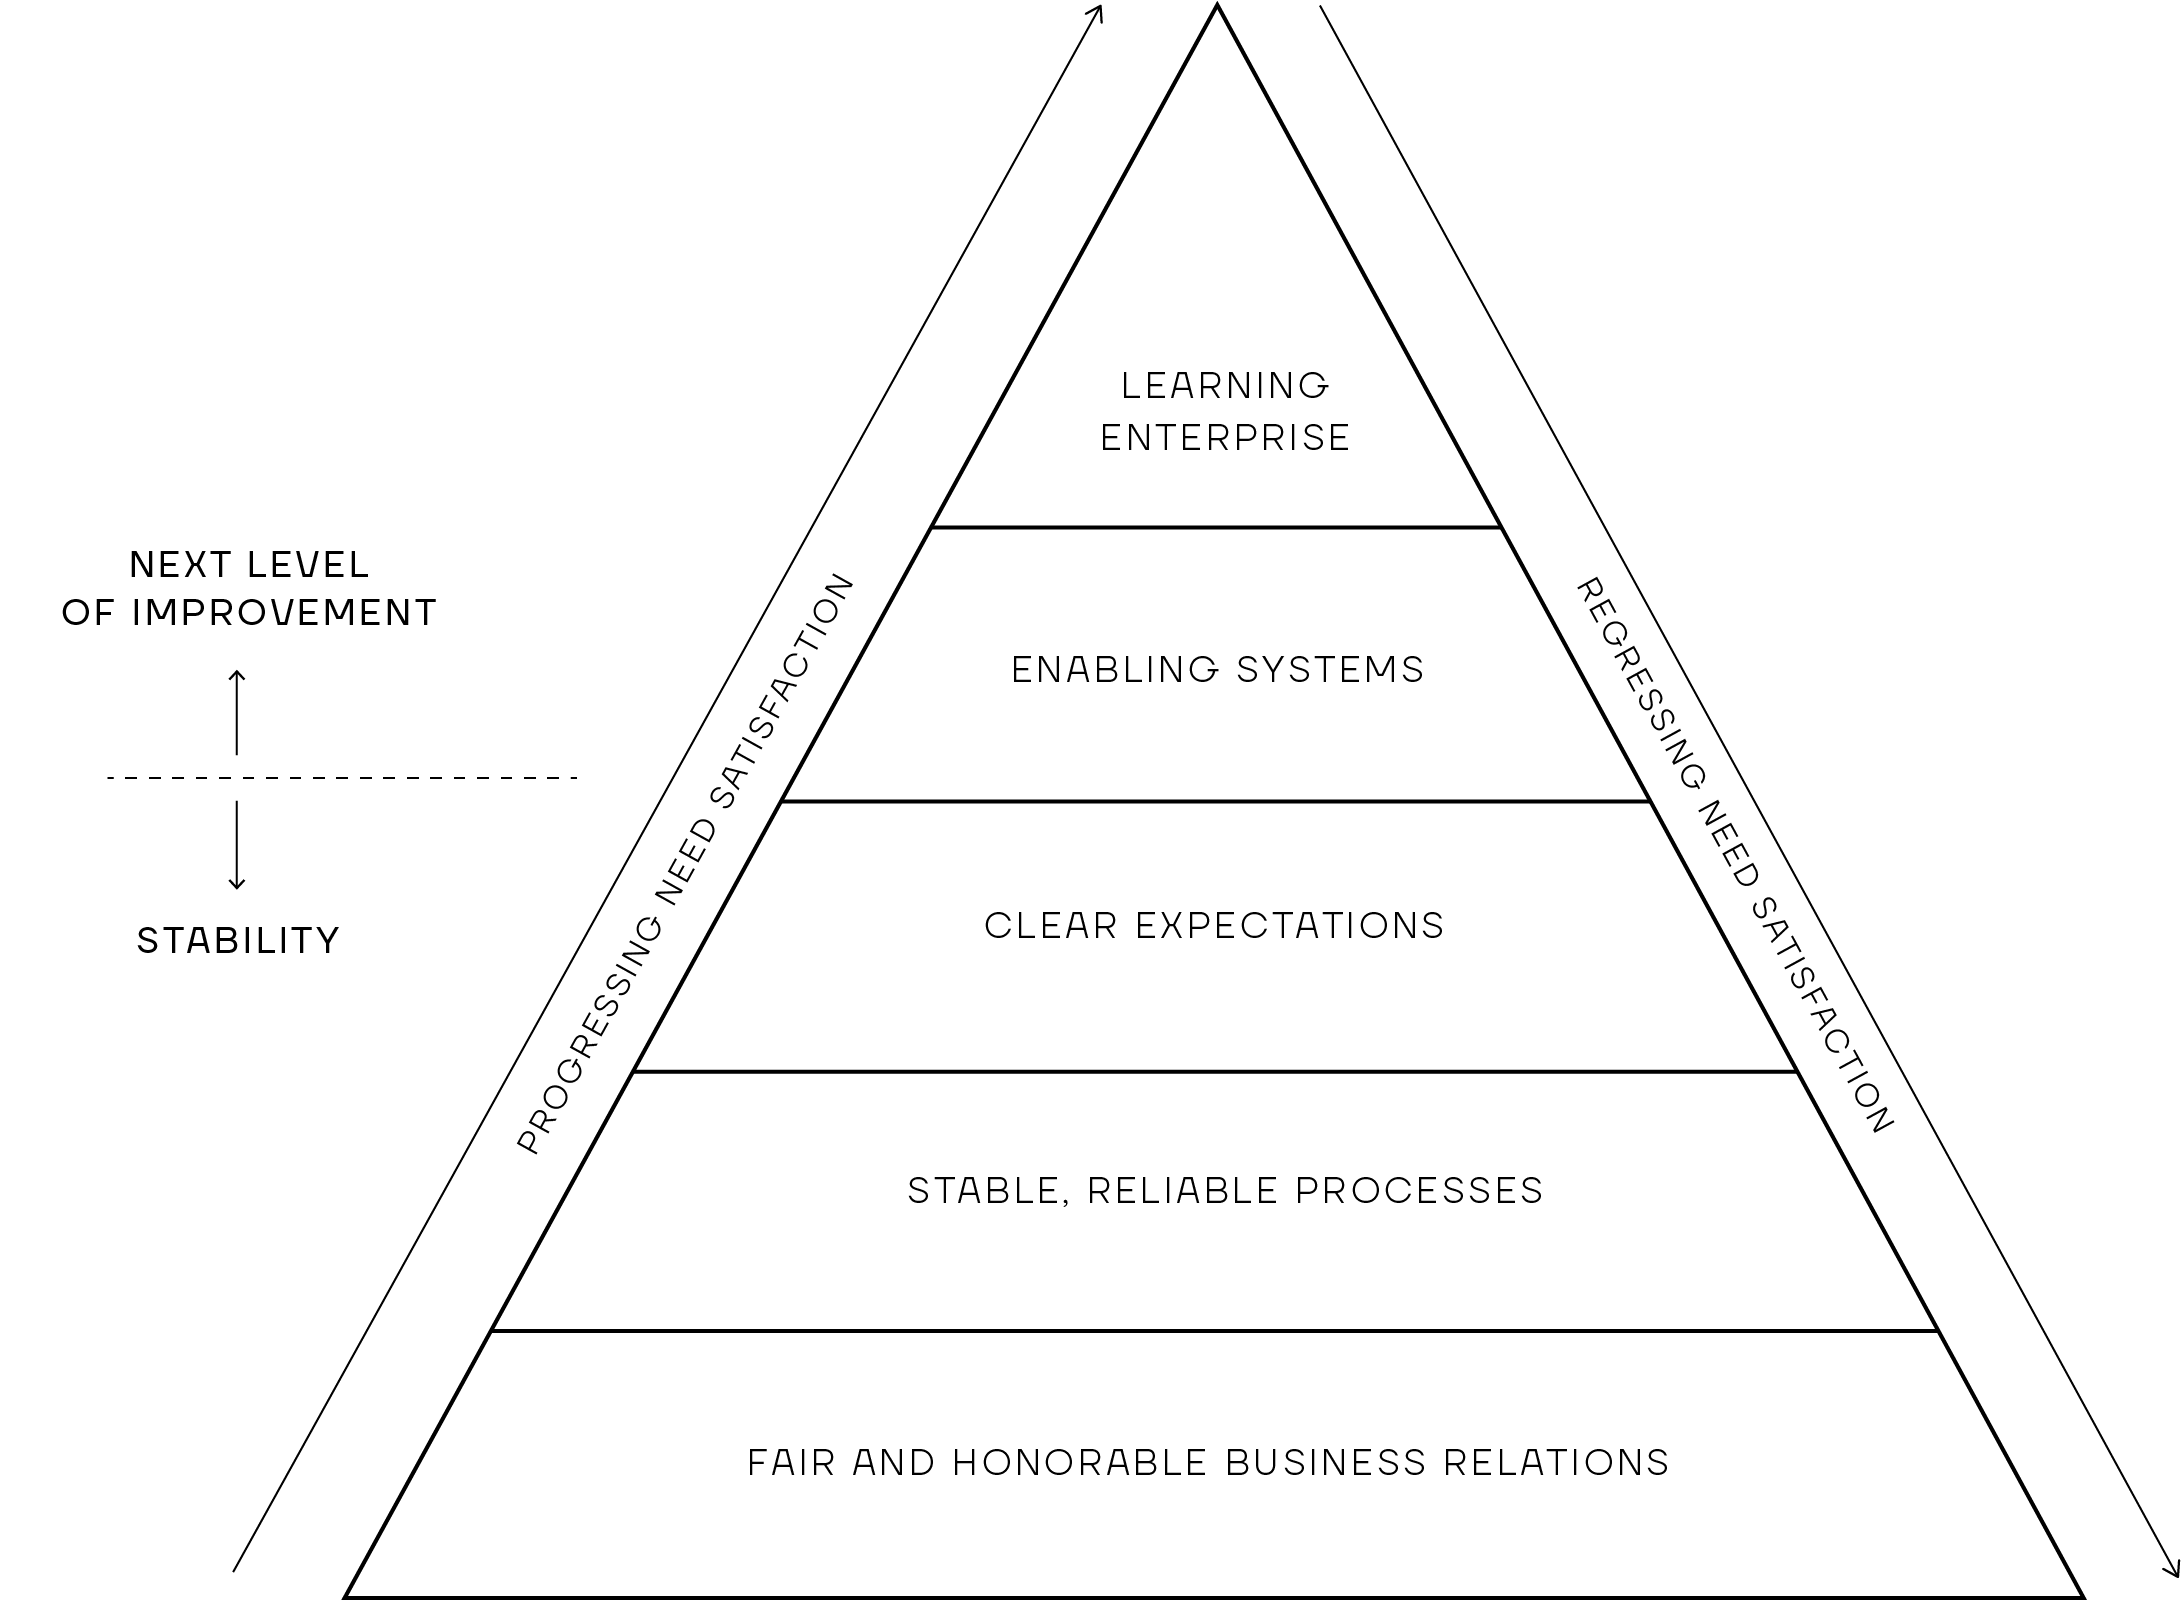
\includegraphics[width=0.7\textwidth]{Netzwerk.png}
  \caption{Supply chain hierarchy of needs}
  \label{Netzwerk}
\end{figure}


\subsection{Problem solving}

The last category is problem solving. Toyota's biggest goal is to become a learning company. The individual principles that help Toyota achieve this are described below.

\subsubsection{12. Principle: Genchi Genbutsu}

Genchi Genbutsu states that to understand the problem comprehensively, you should see for yourself on the ground. A good and famous example is the Ohno circle. Ohno was the plant manager who developed the Toyota Production System. He gave his employees the task of drawing a circle on the floor to stand inside for a day and look at the processes up close. This gave them a very good picture of what was going wrong. Liker describes the approach to observing Toyota as follows:

\begin{itemize}
    \item Always keep the end goal in mind
    \item Plan carefully toward your end goal
    \item Make sure meetings serve a clear purpose
    \item Assign clear tasks to yourself and others
    \item Think and speak based on verified, reliable information and data
    \item Make sure the facts are correct in person
    \item You are responsible for the information you give to others
    \item Share your information with others in a timely manner
    \item Always remember who will benefit from this information
    \item Understand your deficits and competencies in a measurable way
    \item Clarify what knowledge you need to develop yourself further
    \item Strive relentlessly to implement kaizen measures
    \item Think outside the box
    \item Always take care to protect your health and safety
\end{itemize}

\subsubsection{13. Principle: Nemawashi}

The 13th principle is Nemawashi. This has the principle that they should make decisions wisely and according to the consensus principle. One should carefully consider all alternatives, but implement the decision made expeditiously. In the decision-making process, one originally assumes 5 steps:

\begin{enumerate}
    \item Determination of the current situation
    \item knowing and understanding the current factors
    \item consideration of a wide range of alternatives
    \item building consensus within the team
    \item Use of highly effective communication tools
\end{enumerate}

According to Liker, Toyota is once again taking an alternative route. This can be seen in Fig. \ref{Entscheidung}.


\begin{figure}[h] 
  \centering
     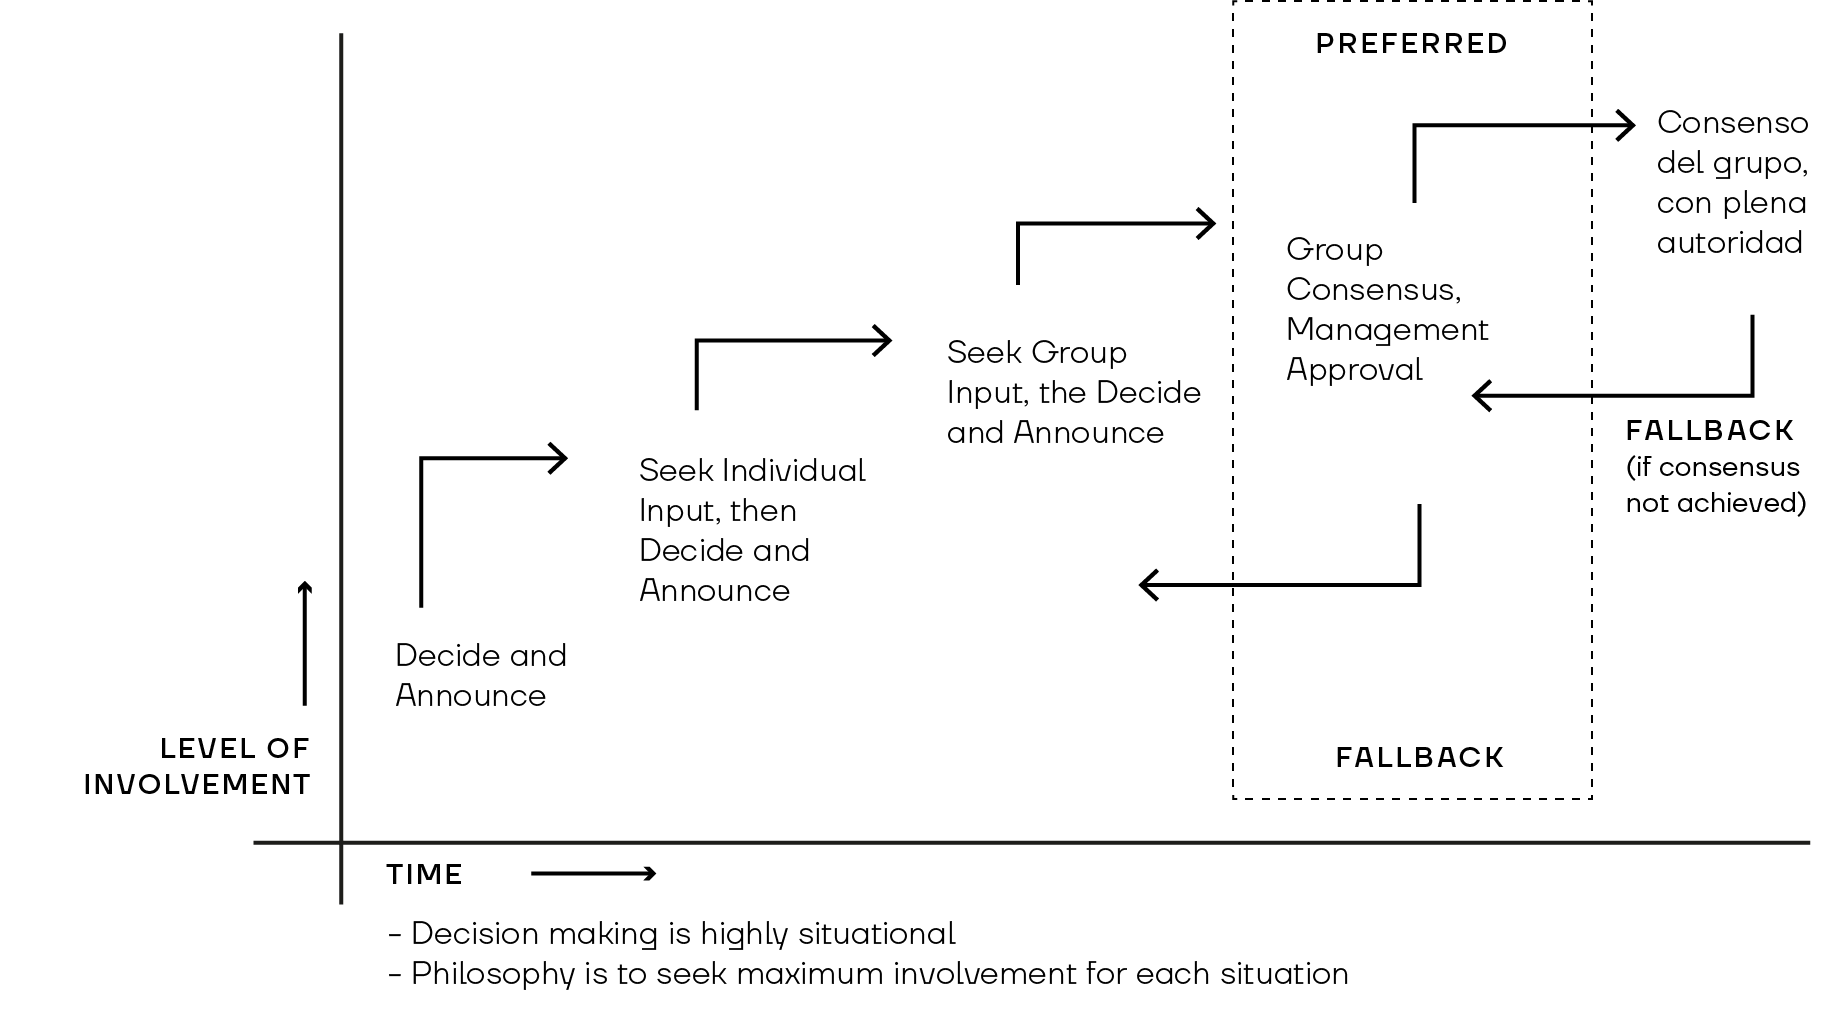
\includegraphics[width=0.6\textwidth]{Entscheidung.png}
  \caption{Toyota's path to decision making}
  \label{Entscheidung}
\end{figure}

\clearpage

Meetings are also an important tool for decision-making. Of course, Toyota has also established some rules for this:

\begin{enumerate}
    \item Clear objectives before the meeting. These objectives can be reflected in the agenda, but the agenda must be very focused on clearly defined tasks and deliverables.
    \item The right audiences must attend. The people who are needed at the meeting must show up.
    \item Prepared participants. All participants know what they need to prepare for the meeting and have done their homework.
    \item Effective use of visual reinforcers. The A3 format is extremely effective.
    \item Separation of information sharing and problem solving. There needs to be as much information sharing as possible before the meeting so that participants can focus on problem solving during the meeting.
    \item The meeting starts and ends on time.
\end{enumerate}

As a result, Toyota achieves an extraordinary collection of information that contributes to decision-making. The advantages of this are obvious. For one thing, it uncovers all the facts, the disregarding of which can cause a lot of trouble at a later stage of the decision-making process and lead to the rewinding of certain steps. In addition, the execution is usually error-free. Toyota involves all affected parties and gains their support of the decision, so that possible resistance can be eliminated before implementation. The cost of overcoming resistance in the implementation phase would in all likelihood be much higher than in the planning phase. Toyota completes a learning process even before the actual planning and implementation.

\subsubsection{14. Principle: Kaizen and Hansei}

The last principle is called kaizen and hansei. These terms mean to become a truly learning organization through relentless reflection (hansei) and continuous improvement (kaizen). Hansei is a cultural thing that is often used in Japan. It involves taking a critical look at one's own performance. To this end, Toyota holds reflection meetings in which the employee discusses his or her own performance with his or her manager. Kaizen describes the continuous improvement, Toyota uses the scheme from Fig. \ref{Problem} to solve its problems. 

\clearpage

\begin{figure}[h] 
  \centering
     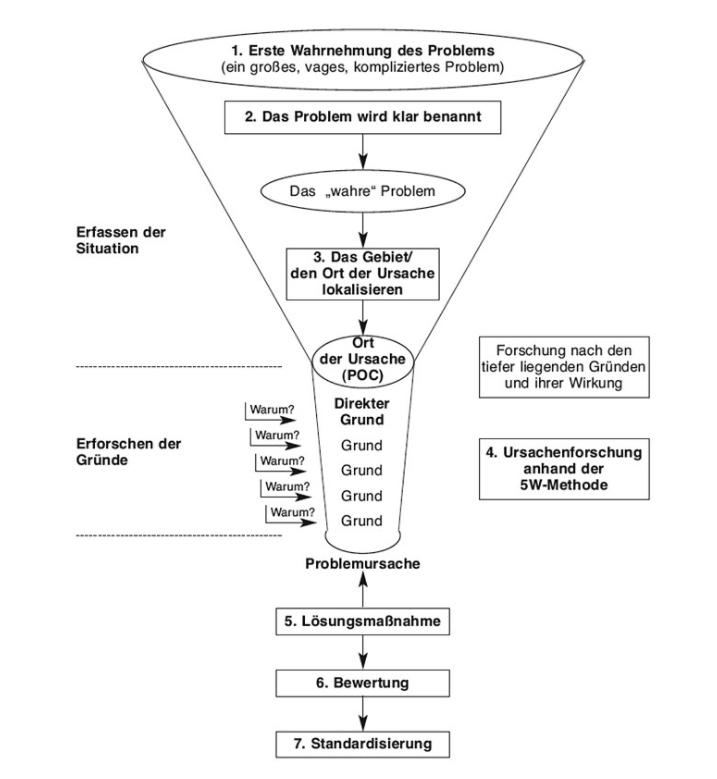
\includegraphics[width=0.5\textwidth]{Problem.png}
  \caption{Toyota's practical problem-solving process}
  \label{Problem}
\end{figure}

The 7 steps are intended to ensure long-term remediation of the problem. To measure the improvements in the company, Liker describes 3 metrics that Toyota looks at:

\begin{enumerate}
    \item Global Performance
    \item Operational performance
    \item Ambitious improvement targets
\end{enumerate}

All these things now lead to creating a flow that enables Toyota to become a learning company. In this process, problems are constantly uncovered, solved, evaluated and integrated into the workflow.

\clearpage
  
\section{Conclusion}

The interaction of all these principles and tools makes Toyota the most successful car manufacturer in the world. It is not about the individual improvements but about the mentality of continuous improvement and the interaction of all points and employees. In fact, Toyota sees respect for people as the most important point of its agenda. I find that the interplay of principles and Toyota's holistic approach creates an atmosphere that provides enough structure for productivity, but also leaves enough room for creative development. 

\clearpage
\addcontentsline{toc}{section}{References}
\begin{thebibliography}{99}

% For books
\bibitem{toyota_book} Jeffrey K. Liker \emph{Der Toyota Weg; 14 Managementprinzipien des weltweit erfolgreichsten Automobilkonzerns}, 8. Aufl. Finanzbuchverlag, München, 2013.


\bibitem{Abbildung 1} Abb. \ref{TPS}: Toyota Produktionssystem \url{https://d2ah727fsr7un8.cloudfront.net/users/154791/154791_FeYuSaDuwoXeyohu9422637115171218.png}, [Online Stand 24.09.2021].

\bibitem{Abbildung 2} Abb. \ref{4P}: 4P Modell des Toyota Weges \url{https://andreasgoetzer.de/wp-content/uploads/Jeffrey-Liker-4P-Modell-TPS-Toyota-Produktionssystem-e1514626930508.jpg}, [Online Stand 24.09.2021].

\end{thebibliography}
\end{document}

